\chapter{Coil design} % Chapter title

\label{ch:coil_design}


\section{Introduction}

Motivation... Where the problem is encountered. Need some citations here.

Coils producing a magnetic field of desired spatial distribution are a necessary ingredient in many engineering and physics applications.

In active magnetic field stabilisation systems the desired field shape is not even known beforehand -- a system capable of producing a aoeu is desired.
The need for coils producing magnetic fields of a desired spatial distribution has
Elaborate methods have been developed, mostly focusing on precision of created field.
Extensive literature to design sophisticated coils.
See an overview by \citeauthor{Turner1993} \citep{Turner1993}.

In particular finds use in active magnetic field stabilisation systems, eg. in nEDM experiments or in PTB (really?).

An interesting approach to coil design was presented by \citeauthor{Compton1982} \citep{Compton1982}. He proposed to divide a surface into small elements and solve for current density in each element. This is very general and powerful idea, albeit the solution is likely to be hard to build.

Most of modern coil design approaches focus on increasing the precision of the created field, giving designs that are very difficult to manufacture. The presented approach focuses on versatility and ease of practical realisation, which makes it potentially useful for large scale builds and systems employing multiple coils.

Mention the main feature of this approach --- the spatial constraint on the location of the wires? Needs some explanation probably.

We begin by presenting a method to describe a subset of all possible coils that can be built on a surface on a square. Next we show how this can be used on a cube to describe coils around a volume. With this algebraic language the coil design is simplified to solving one linear least--squares problem.


\section{Model}
\subsection{Coils as a linear space}
Consider all possible coils that can be constructed by laying wires on a surface of a square. The possibilities are as endless as they are hard to grasp mathematically. What is presented is a language that makes this problem suprisingly simple.

Coils can be seen an vectors in a linear space. One coil spans a one--dimensional space of magnetic fields it can produce. Adding a second coil creates a system spanning a two--dimensional space of fields, thanks to the magnetic field being additive. Four square coils tiled to form a larger square form a four--dimensional space, which is a subset of coils possible to construct on the larger square's surface. This size of the subset we restrict ourselves to is controlled by $N$ --- the number of \emph{base coils} forming the grid. Any coil, member of the subset, is fully described by a vector of $N$ relative currents in each of the \emph{base coils} --- denoted by $\mathbb{I}$. The problem of coil design is thereby simplified to finding a vector $\mathbb{I}$ in a linear space.
% The four coils form a complete linear basis of coils on the surface for any coils that have wires going only along the edges --- see Fig.\,\ref{fig:coils_tile_basis}. This is a very convenient subspace of all coils possible to build on a square. The possible to realise subspace may be enlarged by refining the division into tiles. But as a coil is equivalent to the field it produces, one can just as well say that they form a four--dimensional \emph{space of coils}.

\begin{figure}[bth]
  \myfloatalign
  \subfloat[A basis of four base--coils on a surface. Three vectors are presented together with their explicit coordinates in the basis.]
  {\label{fig:coils_tile_basis}
  \includegraphics[width=.45\linewidth]{gfx/tile_basis}}
  \quad
  \subfloat[A coil which spans one--dimensional subspace of coil--vectors on a cuboid that produces no magnetic field.]
  {\label{fig:coils_tile_kernel}
  \includegraphics[width=.45\linewidth]{gfx/tile_kernel}}
  \caption{Coils as a vector space.}
\end{figure}

A cube consists of six square faces. Therefore the set of \emph{base coils} can be constructed by dividing each face into a grid. However, for a set of $N$ grid coils the space of fields possible to produce has dimension $N-1$. Consider six square coils combined into a cube form only a five--dimensional space of coils, as same current flowing in each of the coils produces no field, as explained in Fig.\,\ref{fig:coils_tile_kernel}. Dividing the faces of the cube into $N$ tiles provides a simple basis for many coils that can be built around a volume.

% A cube consists of six square faces. On each a grid may be constructed, forming a set of $N$ \emph{base coils}.  smaller The problem of coil design is much simpler, as now it is a problem in a finite--, $N$--dimensional linear space. A $coil$ is fully described by a set of $N$ currents in each of the \emph{base coils} --- $\mathbb{I}$. At the cost of restraining oneself to coils that can have wires only along the edges of the tiles, one gains a tremendous simplification of the problem.
% However, six square coils combined into a cube form only a five--dimensional space of coils, as same current flowing in each of the coils produces no field, as explained in Fig.\,\ref{fig:coils_tile_kernel}. Dividing the faces of the cube into $N$ tiles provides a simple basis for many coils that can be built around a volume.

The mechanical constrain can be of tremendous advantage. Every coil in this subspace is guaranteed to be mechanically constrained to the edges of the tiles. Once a mechanical support is build, coil may be designed and added even later.

In a coil constructed in the presented scheme in general a lot of currents, flowing in an opposite direction along the same edge, would cancel. For each edge there are two adjacent \emph{base coils}, so inevitably some currents will, at least partially, cancel. A coil can always be simplified by simply adding the two currents flowing along each edge, as it is presented in Fig.\,\ref{fig:coils_tile_basis}.


\subsection{Coil design}
In the problem of coil design one wants to create \emph{a coil that will best approximate a given field in a certain volume}. Let us call this volume \emph{the volume of interest}. It can be of an arbitrary shape and is located fully inside the coil system (the cube). One can pick an ensemble of $n$ points on the surface of the \emph{volume of interest} (its surface is sufficient because $\nabla \mathbf{B} = 0$). Let us denote the combined vector, dimension $3n$, of magnetic field in each of the point by $\mathbb{B}$.

% Note, that magnetic field produced by a coil at a given point in space is proportional to the current in this coil. For a fixed direction in a fixed point in space it is a linear combination of currents of all coils in the system. Now, if we consider a vector of 3 spatial directions in $M$ points \ie, dimension $3M$. It can be obtained from an arbitrary coil $C$ by multiplying it by a $NNN \times 3M$ matrix $\mathbb{M}$. This matrix encodes the geometry of the system and may be pre-calculated.

Note, that magnetic field produced by a coil at a given point in space is proportional to the current in this coil. For a fixed direction in a fixed point in space it is a linear combination of currents of all coils in the system. In an absence of external magnetic field the system is thus described by a simple linear equation:
\begin{equation}
  \mathbb{B} = \mathbb{M} \, \mathbb{I}
\end{equation}
where $\mathbb{M}$ is a $3n \times N$ matrix encoding the geometry of the system.

For rectangular tiles the matrix can be easily calculated using the formula given by \citeauthor{Reta-Hernandez1998}~\citep{Reta-Hernandez1998}). If the tiles are not rectangular then it can still be analytically obtained by integration of the Biot--Savart law.

The goal is to design a coil that would best approximate a field $\mathbf{B}_0$ in the \emph{volume of interest}. In the $n$ points of interest the field has values $\mathbb{B}_0$ --- a vector similar to $\mathbb{B}$. The \emph{coil} is evaluated by solving the following linear problem for $\mathbb{I}$:
\begin{equation}
  \mathbb{M} \, \mathbb{I} \stackrel{!}{=} \mathbb{B}_0
\end{equation}
If one picks enough points that $\mathrm{dim}(\mathbb{B}) > \mathrm{dim}(I)$, then the equation is an over--determined set of linear equations. The solution is found by the ordinary least--squares method.

Solving the least--squares problem will produce for \emph{any} field $\mathbf{B}_0$
\emph{the} optimal coil in the restricted space. I emphasise, that the spatial restriction is
may be highly desirable. Especially if a number of coils, each producing different field, is to be would around the volume. In the presented scheme adding a new coil will not cover the \emph{surface of the coils} more densely, as opposed to other schemes in the literature.

\subsection{Examples}
The simplest magnetic field is a homogeneous one. Figures\,\ref{fig:coils_homogeneous_3d} and \ref{fig:coils_homogeneous_section} show a coil designed for the homogeneous field. The \emph{coil surface} is a $\unit[1]{m^3}$ cube, the \emph{volume of interest} is a $\unit[0.75^3]{m^3}$ cube. The cube has been divided into $5 \times 5 \times 6 = 150$ tiles. The system achieves a 2\% homogeneity in the whole \emph{volume of interest}.

The full power of this scheme is visible, when the desired $B_0$ field is complicated. One may want to counteract a fixed nearby dipole source. A coil designed for that is presented in Fig.\,\ref{fig:coils_dipole_3d}.

\begin{figure}[bth]
  \myfloatalign
  \subfloat[A coil designed for a homogeneous $50\,\mathrm{\micro T}$ field along the x--axis. A net current along each edge is shown.]{
    \label{fig:coils_homogeneous_3d}
    \includegraphics[width=.45\linewidth]{gfx/coil_homogeneous}}
  \quad
  \subfloat[XY section in the middle --- achieved relative compensation of the homogeneous field.]{
    \label{fig:coils_homogeneous_section}
    \includegraphics[width=.45\linewidth]{gfx/coil_homogeneous_section}}
  \\
  \subfloat[A coil designed for a dipole disturbance, $3\,\mathrm{kNm/T}$, $2.2\,\mathrm{m}$ away from the centre with 5x5 base tiles per face.]{
    \label{fig:coils_dipole_3d}
    \includegraphics[width=.45\linewidth]{gfx/coil_dipole}}
  \quad
  \subfloat[XY section in the middle --- achieved relative compensation of the homogeneous field.]{
    \label{fig:coils_dipole_section}
    \includegraphics[width=.45\linewidth]{gfx/coil_dipole_section}}
  \caption{Coils as a vector space.}
\end{figure}


\section{A good set of coils for an arbitrary field}
When one wants to be able to produce an arbitrary field, it is best to use an orthogonal expansion, in analogy to the Taylor expansion for functions. Furthermore, it is desired that the terms of the expansions are natural for the system considered (as spherical harmonics used to describe the wavefunctions of electrons in atomic systems are solutions to the Schrödinger equation themselves). Also, from the point of view of control, it is much easier to control an orthogonal system. See eg. \,\citep{Branch1984} for detailed motivation (really?). In an expansion one can gradually improve the system.

Such an expansion exists: \emph{carthesian harmonic polynomials}.
\begin{equation}
  \mathbf{B}(\mathbf{r}) = \sum_{n}\,H_n\mathbf{P}_n(\mathbf{r})
\end{equation}
where $H_n$ are the expansion coefficients. They satisfy Maxwell's equations, so it is always theoretically possible to create a coil that produces the eigenfunctions. The table~\ref{tab:coils_carthesian_harmonics} presents first few of them.

\begin{table}
  \centering
  \begin{tabular}{c|ccc}
    n & $P_n^x(\mathbf{r})$ & $P_n^y(\mathbf{r})$ & $P_n^y(\mathbf{r})$ \\ \hline
    1 & 1 & 0 & 0 \\
    2 & 0 & 1 & 0 \\
    3 & 0 & 0 & 1 \\ \hline
    4 & $x$ &  0  & $-z$ \\
    5 & $y$ & $x$ &   0  \\
    6 &  0  & $y$ & $-z$ \\
    7 & $z$ &  0  & $ x$ \\
    8 &  0  & $z$ & $-y$ \\
  \end{tabular}
  \label{tab:coils_carthesian_harmonics}
  \caption{Carthesian harmonic polynomials.}
\end{table}

The first three terms are homogeneous fields. Further five are the five independent gradients.


\section{Construction}
The first step is to define the \emph{coil surface}. Afterwards the surface has to be divided into tiles. The tiles need not necessarily be squared. They may not be rectangular, on even not flat. The finer the division, the better the field can be approximated, but also the harder it is to construct the system. A simple choice is to choose the coil surface to be a cuboid and the tiles to be rectangles.


Exploit symmetries --- a homogeneous coil may be viewed a sum of a number of
much simpler to construct coils, which are then connected in series.

\begin{figure}[bth]
  \myfloatalign
  \includegraphics[width=.6\linewidth]{gfx/coils/wiring}
  \caption
  [TODO]
  {%FIXME directly copied from the SFC paper
The wiring solution.}
  \label{fig:coils_wiring}
\end{figure}

Each edge can have any real current (albeit the Kirchoff law is fulfilled).
However, to keep the number of control channels reasonably small, they need
to be driven with one current source. Two techniques may be used:
\begin{enumerate}
  \item using a different number of wires, connected in series --- only discrete
  \item varying resistance of different parts of the coil connected in parallel
  --- can be adjusted continuously, but causes power dissipation.
\end{enumerate}

1A, 0.1A, 0.001A wires solution --- keeps the number of windings reasonably small.
With a simple use of additional resistors each coil may be still driven with only
one power supply --- \emph{provide a figure}.

\begin{figure}[bth]
  \myfloatalign
  \includegraphics[width=.6\linewidth]{gfx/coils/current_discretisation}
  \caption
  [TODO]
  {%FIXME directly copied from the SFC paper
The wirining solution.}
  \label{fig:coils_current_discretisation}
\end{figure}

Care has to be taken to balance voltage and current needs for the power supplies.

Parameters to vary: number of windings, thickness of cable (price). Note also
the inductance of the coils.

\subsection{Possible generalisations}
\begin{enumerate}
  \item the surface does not need to be cubic
  \item
\end{enumerate}



\section{Practical application --- SFC system}
\subsection{Surrounding Field Compensation in the nEDM experiment}
The main challenge of the nEDM experiment is reaching a magnetic field stability on the picotesla level on a timescale of minutes. At the same time the experiment is set up in a research facility, where strong magnets are common. In fact, at the experimental site the compass points in different directions throughout the day.

The main part of attenuation of the magnetic field is done by four layers of \mbox{μ-metal} --- material with very high permeability (around 400\,000). However, \mbox{μ-metal}, being a ferromagnetic, is itself susceptible to become magnetised and and create a magnetic field of its own. In order to keep the magnetisation stable the \mbox{μ-metal} shield has been surrounded by a system of large coils. The coils are driven in a feedback loop with magnetic filed sensors (see Fig.\,\ref{fig:nEDM_SFC}). The system has been described in the paper \citep{Afach2014}.

\begin{figure}[bth]
  \myfloatalign
  \includegraphics[width=.6\linewidth]{gfx/nEDM_SFC}
  \caption
  [Sketch of the nEDM SFC system.]
  {%FIXME directly copied from the SFC paper
Sketch of the SFC system consisting of six coils surrounding the Mu-metal magnetic shield of the nEDM spectrometer. The visible outermost layer of the cylindrical shield is mounted in its aluminum support structure.
The Helmholtz coil pairs are labeled (X+, X-),(X-, Y-) and (Z+,Z-). The coordinate system of the experiment is given at the lower right. Its origin is at the center of the magnetic shield. Three--axis fluxgates (open circles) are mounted on the aluminium support of the experiment and numbered according to the fluxgate nomenclature given in the text. The positions 10 and 50 (full circles) depict previous locations of fluxgates FG 1 and FG 5 referred to in Sec. VB. FG 4 is omitted as it was removed from the system after a sensor failure.}
  \label{fig:nEDM_SFC}
\end{figure}

The SFC system operates since 2013, attenuating the magnetic field by factor more than 5, even during ramping of nearby magnets.


\subsection{Design for n2EDM}

The volume is cubic.

The SFC system is going to be very large --- $\unit[6x6x6]{m^3}$. Elaborate designs, such as wires of variable length, or arbitrarily bended wires would be complicated to realise in such scale.

Moreover, the system is going to enclose the whole apparatus.
Super crucial --- many coils on the same surface 3 for the first order compensation, but then 9 for gradients. That is already 12 coils. If one only restrict oneself to a surface, it is guaranteed to end up with it densely covered with wires. In this approach the geometry is limited by design.

Mention, that the \micro-metal presence does not disturb much, as it is already placed in a small field.


Design goals / challenges:
\begin{enumerate}
  \item Better shielding factor. Attenuation by a factor of 50 in the whole volume of the shield. The design goal has been set to reach at most 2\% of the ambient magnetic field in the
  whole volume of the experiment. In \unit[50]{\micro T} this corresponds to a nice value of \unit[1]{\micro T}.
  \item Very large fiducial volume --- due to spatial constrains of the experimental site --- biological shielding. PUT IMAGE!!! Not only is the compensation expected to be better, but also provide a much larger volume. Next version of the experiment --- much larger.
  \item As is nEDM --- many coil system. But orthogonal, or at least close to one. Three coils for compensating the three homogeneous components of the magnetic field. Then 9 for gradients. The strongest fields are low--order, and only these require strong compensation coils (thick wires, big and expensive power supplies). The higher--order coils may be constructed with thinner wires and cheaper power supplies.
  Additionally, this makes the control of the system simpler.
  This also states the problem better. One has to design and construct coils that create homogeneous field in the volume occupied by the shield. Maybe elaborate more on the field decomposition!
  \item Coil tailored for the specific magnetic environment of the n2EDM site. Coils tailored for nearby magnets.
\end{enumerate}


\section{Prototype}
A comprehensive setup for prototyping magnetic field related systems for n2EDM has been designed and is, as of today, under construction. Its main part is a scaled--down model of the outermost layer of n2EDM µ-metal shield. Design of a degaussing and SFC systems for the setup is ongoing. In the future the setup can host also a prototypes of an internal magnetic field mapper, a main holding--field coil and, possibly, other systems.

\subsection{Maps}

\section{Potential problems}
\begin{enumerate}
  \item The numerical problem of subtracting numbers.
  \item The discretisation is happening twice --- first is the division into tiles. Then the current in the solution needs to be discretised too.
\end{enumerate}
